\chapter{Renormalized Operators and Minimal Subtraction}
\label{ch:volume-ii-renormalized-operators-minimal-subtraction}
\ConventionsEuclidean


\section{Operators from Infinitesimal Deformations}

The 1PI renormalization group compares scale-dependent coordinates
\(g_I(\mu)\) on a renormalized family of theories.  Local operators enter the
same structure through infinitesimal deformations of the action.  Fix a finite
or graded local operator basis \(\{O_I\}_{I\in\mathcal I}\), chosen so that
operators with the same spacetime and internal quantum numbers are included
together whenever perturbation theory can mix them.  To define insertions as
distributions, first allow smooth compactly supported source functions
\(\eta_0^I(x)\) and write
\[
  \delta S_\eta
  =
  \int \dd^D x\,\eta_0^I(x)\,O_I(x).
\]
Constant sources \(\eta_0^I(x)=\delta g_I\) give the deformation
\[
  \delta S
  =
  \int \dd^D x\,\sum_I \delta g_I\,O_I(x).
\]
Here \(\delta g_I\) are bare deformation coefficients.  At scale \(\mu\), the
same deformation can be described by renormalized source functions
\(\eta_\mu^J(x)\).  Linearity in the infinitesimal source gives a matrix
\(N_{JI}(\mu)\) such that
\[
  \eta_0^I(x)
  =
  \sum_J\eta_\mu^J(x)\,N_{JI}(\mu).
\]
For constant sources this becomes
\[
  \delta g_I
  =
  \sum_J\delta g_J(\mu)\,N_{JI}(\mu).
\]
Substituting this into \(\delta S\) gives
\[
  \delta S
  =
  \int \dd^D x\,\sum_J \delta g_J(\mu)
  \left(\sum_I N_{JI}(\mu)\,O_I(x)\right).
\]

\begin{definition}[Renormalized local operator]
In the deformation chart above, the renormalized operator associated with the
source coordinate \(\eta_\mu^I\), or equivalently with the coupling
coordinate \(g_I(\mu)\) for constant sources, is
\[
  [O_I]_\mu
  =
  \sum_J N_{IJ}(\mu)\,O_J .
\]
Equivalently,
\[
  \delta S
  =
  \int \dd^D x\,\sum_I \delta g_I(\mu)\,[O_I]_\mu(x).
\]
The matrix \(N_{IJ}(\mu)\) is part of the renormalization scheme.  Its rows
label renormalized deformation coordinates, and its columns label the chosen
bare operator basis.  As an insertion in correlation functions, the equality
is an equality of distributions away from coincident points; different
renormalization prescriptions for contact terms differ by local terms
supported on collision diagonals, in the sense of
Definition~\ref{def:contact-terms-source-chart}.
\end{definition}

\section{Operators as Cotangent Data}

\begin{warning}[\(\gamma\)-indices]
Throughout this chapter the anomalous-dimension matrix for deformation
operators is indexed in the cotangent convention
\[
  \frac{\dd}{\dd\log\mu}[O_I]_\mu
  =
  -\gamma_{IK}[O_K]_\mu,
  \qquad
  \gamma_{IK}
  =
  \frac{\partial\beta_K}{\partial g_I}.
\]
Thus the first index labels the source or coupling coordinate dual to the
operator being differentiated, and the second index labels the operator
appearing after the cotangent action.  Many column-vector conventions in the
physics literature denote the same Jacobian component by
\[
  \gamma^{\rm col}_{KI}
  =
  \frac{\partial\beta_K}{\partial g_I}
  =
  \gamma_{IK}.
\]
Comparisons of formulae must therefore transpose this pair of labels.
\end{warning}

The preceding definition has a geometric interpretation.  The infinitesimal
coupling displacement
\[
  \delta g=\delta g_I\,\frac{\partial}{\partial g_I}
\]
is a tangent vector to the renormalized family of theories.  The corresponding
local operator insertion is the dual object specified by the pairing
\[
  \langle \delta g,O\rangle
  =
  \int \dd^D x\,\delta g_I\, [O_I]_\mu(x).
\]
The deformation \(\delta S\) is this pairing.  Therefore a change of
renormalized coordinates
\[
  \widetilde g_A=f_A(g)
\]
must transform the operator representatives by the inverse Jacobian:
\[
  [\widetilde O_A]_\mu
  =
  \frac{\partial g_I}{\partial \widetilde g_A}\,
  [O_I]_\mu .
\]
This is the cotangent transformation law, with the Jacobian evaluated at the
theory point under consideration.  It is the local-operator version of the
statement that beta functions are components of a vector field.  The statement
applies to the deformation operators dual to the selected coordinate chart;
additional local operators may require enlarging the chart before their mixing
can be described by the same matrix.

\begin{definition}[Deformation-operator bundle]
\label{def:deformation-operator-bundle}
Let \(U\) be a coordinate neighborhood in the finite-dimensional
renormalized theory space with coordinates \(g_I\).  The
\emph{deformation-operator bundle} over \(U\) is the vector bundle
\(\mathcal E_{\rm def}\to U\) whose local representative column over the chart
\(g\) is the ordered family of source-normalized insertion distributions
\[
  e_I(g,\mu)=[O_I]_\mu .
\]
Its fiber at \(g\) is the span of the deformation operators dual to tangent
vectors \(\partial/\partial g_I\), with equality of insertions understood on
noncoincident test configurations and with a separately specified contact-term
extension.  On an overlap with coordinates \(\widetilde g_A=f_A(g)\), the
transition functions are specified in the convention that local representative
columns transform by \(v_{\widetilde g}=M_{g\to\widetilde g}v_g\).  The
operator column therefore obeys
\begin{equation}
  \widetilde e_A
  =
  M_{AI}(g)\,e_I,
  \qquad
  M_{AI}(g)=\frac{\partial g_I}{\partial\widetilde g_A}.
  \label{eq:deformation-operator-bundle-transition}
\end{equation}
Thus, for deformation operators, \(\mathcal E_{\rm def}\) is the source-defined
realization of \(T^*U\).  If one includes local operators not dual to coupling
coordinates, the same construction gives a larger operator bundle only after a
finite-rank source chart and its transition functions have been specified.
\end{definition}

Let \(t=\log\mu\).  The tangent vector \(\delta g_K\) evolves by the
linearized RG equation
\[
  \frac{\dd}{\dd t}\delta g_K
  =
  \frac{\partial\beta_K}{\partial g_I}\,\delta g_I .
\]
Scale independence of the bare deformation means that the pairing
\(\langle\delta g,O\rangle\) is independent of \(t\).  Hence the dual operator
basis evolves with the negative transpose action:
\[
  \frac{\dd}{\dd t}[O_I]_\mu
  =
  -
  \frac{\partial\beta_K}{\partial g_I}\,[O_K]_\mu .
\]
The index placement in the anomalous-dimension matrix below is chosen to
encode precisely this cotangent action.

The scale dependence of \(N_{IJ}\) follows from the scale independence of the
bare deformation.  Let
\[
  \frac{\dd g_I(\mu)}{\dd\log\mu}
  =
  \beta_I(g(\mu))
\]
be the beta functions of the underlying finite-dimensional coordinate system.
For an infinitesimal displacement \(g_I(\mu)\mapsto g_I(\mu)+\delta g_I(\mu)\),
the beta function changes by
\[
  \delta\beta_K
  =
  \sum_I
  \frac{\partial\beta_K}{\partial g_I}\,\delta g_I(\mu).
\]
Define the anomalous-dimension matrix in this deformation convention by
\[
  \gamma_{IK}(g)
  =
  \frac{\partial\beta_K}{\partial g_I}(g).
\]
Differentiating
\(\delta g_I=\sum_J\delta g_J(\mu)N_{JI}(\mu)\) with respect to
\(\log\mu\) and using the preceding linearized flow gives
\[
\begin{aligned}
  0
  &=
  \frac{\dd\,\delta g_I}{\dd\log\mu}                                      \\
  &=
  \sum_J
  \left[
    \delta\beta_J(g(\mu))\,N_{JI}(\mu)
    +
    \delta g_J(\mu)
    \frac{\dd N_{JI}(\mu)}{\dd\log\mu}
  \right]                                                                  \\
  &=
  \sum_{J,K}
  \delta g_K(\mu)\,
  \frac{\partial\beta_J}{\partial g_K}(g(\mu))\,N_{JI}(\mu)
  +
  \sum_J
  \delta g_J(\mu)\,
  \frac{\dd N_{JI}(\mu)}{\dd\log\mu}.
\end{aligned}
\]
Since the infinitesimal renormalized displacement \(\delta g_J(\mu)\) is
arbitrary, this is equivalent to
\[
  \frac{\dd N_{IJ}}{\dd\log\mu}
  =
  -\sum_K \gamma_{IK}(g(\mu))\,N_{KJ}(\mu).
\]
Consequently the renormalized operators satisfy
\[
  \frac{\dd}{\dd\log\mu}[O_I]_\mu
  =
  -\sum_K\gamma_{IK}(g(\mu))\,[O_K]_\mu .
\]

Figure~\ref{fig:volume-ii-operator-mixing-field} records the two pieces of data
entering this equation: operator mixing among the chosen local basis and field
renormalization on the external legs of insertion kernels.

\begin{figure}[H]
  \centering
  \resizebox{0.96\textwidth}{!}{%
  \begin{tikzpicture}[x=1cm,y=1cm,every node/.style={font=\scriptsize}]
    \begin{scope}
      \node[font=\small] at (0,2.25) {operator mixing};
      \draw[thick] (-2.1,-0.2) rectangle (0.95,1.45);
      \draw (-1.1,-0.2)--(-1.1,1.45);
      \draw (-0.1,-0.2)--(-0.1,1.45);
      \draw (-2.1,0.35)--(0.95,0.35);
      \draw (-2.1,0.90)--(0.95,0.90);
      \node at (-1.6,1.18) {\(N_{11}\)};
      \node at (-0.6,1.18) {\(N_{12}\)};
      \node at (0.45,1.18) {\(\cdots\)};
      \node at (-1.6,0.63) {\(N_{21}\)};
      \node at (-0.6,0.63) {\(N_{22}\)};
      \node at (0.45,0.63) {\(\cdots\)};
      \node at (-1.6,0.08) {\(\vdots\)};
      \node at (-0.6,0.08) {\(\vdots\)};
      \node at (0.45,0.08) {\(\ddots\)};
      \node[align=center] at (2.35,0.72)
        {\([O_I]_\mu=\)\\[-1pt]\(\sum_JN_{IJ}O_J\)};
      \draw[-{Latex[length=2mm]}, thick] (-1.6,-0.92)--(1.55,-0.92);
      \node[below] at (-1.6,-1.02) {\(\mu'\)};
      \node[below] at (1.55,-1.02) {\(\mu\)};
      \node[blue!70!black, align=center] at (0,-1.55)
        {generated by\\\(\gamma_{IK}=\partial\beta_K/\partial g_I\)};
    \end{scope}

    \begin{scope}[shift={(6.0,0)}]
      \node[font=\small] at (0,2.25) {field insertion};
      \draw[thick] (-2.1,0.55)--(-0.62,0.55);
      \fill[gray!18, draw=black, thick] (0,0.55) circle (0.48);
      \node at (0,0.55) {1PI};
      \draw[thick] (0.48,0.55)--(1.65,0.55);
      \fill[red!75!black] (1.65,0.55) circle (2.4pt);
      \node[red!75!black, above] at (1.65,0.85) {\(\delta g_1\)};
      \node[align=center] at (0,-0.55)
        {amputated insertion\\fixed by field normalization};
      \node[blue!70!black] at (0,-1.35)
        {\([\phi]_\mu=Z(\mu)^{-1/2}\phi\)};
    \end{scope}
  \end{tikzpicture}
  }
  \caption{Renormalized local operators are rows of the mixing matrix
  \(N_{IJ}\).  The matrix evolves with the linearized beta-function vector
  field.  For the elementary field insertion, the running is the same
  wavefunction normalization used in the 1PI coordinate system.}
  \label{fig:volume-ii-operator-mixing-field}
\end{figure}

\section{Source-Extended Wilsonian Representatives}

The preceding discussion used local sources to define renormalized operators
as cotangent vectors to a space of couplings.  The same source coordinates
also have a Wilsonian representative.  The complete construction consists of
three linked objects: a Wilsonian insertion functional, its connected
low-field expectation, and its 1PI Legendre-transform representative.

Work at a finite ultraviolet regulator \(\Lambda_0\), and let
\(\Lambda<\Lambda_0\) be a smooth Wilsonian cutoff.  The regulated field is
decomposed as a sum of an independent low field \(\phi\) with covariance
\(C_\Lambda\) and a shell field \(\phi_{\mathrm{sh}}\) with positive covariance
\(\widehat C_{\Lambda_0,\Lambda}=C_{\Lambda_0}-C_\Lambda\), or with any
equivalent smooth positive covariance decomposition.  The shell kinetic term
\(\widehat S_{\mathrm{kin}}\) is the quadratic form inverse to
\(\widehat C_{\Lambda_0,\Lambda}\) on the regulated vector space.  Choose a
local bare operator basis \(O_I(x)\) and source functions \(\eta_0^I(x)\).  In
the Euclidean sign convention used in this volume,
\[
  Z_{\Lambda_0}[J,\eta_0]
  =
  \int D_{\Lambda_0}^{\rm ref}\phi\,
  \exp\left[
    -S_{\Lambda_0}[\phi]
    -\int\dd^D x\,J(x)\phi(x)
    -\int\dd^D x\,\eta_0^I(x)O_I(x)
  \right].
\]
Here \(D_{\Lambda_0}^{\rm ref}\phi\) is the reference density of
Definition~\ref{def:regulated-scalar-integration-conventions}; the full
quadratic kinetic term is included in \(S_{\Lambda_0}\).  In the Gaussian
form used for the Wilsonian pushforward below, the same finite-regulator
integral is expressed by placing the quadratic form in a centered Gaussian
measure and retaining only the interaction/source functional in the
exponential.
Thus
\[
  -\frac{\delta W_{\Lambda_0}[J,\eta_0]}
          {\delta\eta_0^I(x)}
  \bigg|_{\eta_0=0}
  =
  \bigl\langle O_I(x)\bigr\rangle_{J,\Lambda_0},
  \qquad
  W_{\Lambda_0}=\log Z_{\Lambda_0},
\]
where the expectation value is computed with the source \(J\) still present.
Higher derivatives with respect to \(\eta_0\) give connected insertions, with
the corresponding signs determined by the same convention.

The Wilsonian source coordinates at scale \(\Lambda\) are denoted
\(\eta_\Lambda^A(x)\).  Locality permits a source-coordinate change by a local
linear differential operator,
\begin{equation}
  \eta_0^I(x)
  =
  \bigl(\mathcal Z_\Lambda\bigr)^I{}_A(\partial_x)\,
  \eta_\Lambda^A(x),
  \label{eq:source-coordinate-local-differential-map}
\end{equation}
where
\[
  \bigl(\mathcal Z_\Lambda\bigr)^I{}_A(\partial)
  =
  \sum_{|\alpha|\ge0}
  \bigl(\mathcal Z_\Lambda\bigr)^I{}_{A,\alpha}\,
  \partial^\alpha
\]
as a formal derivative expansion, restricted by the spacetime and internal
quantum numbers of the sources.  For constant sources only the
\(\alpha=0\) term contributes.  The finite matrix \(N_{AI}(\mu)\) introduced
above is the corresponding zero-momentum source-renormalization matrix in a
chosen 1PI coordinate chart.

Define the source-extended Wilsonian interaction \(L_\Lambda[\phi;\eta_\Lambda]\)
by the Gaussian pushforward
\begin{equation}
  \exp\bigl[-L_\Lambda[\phi;\eta_\Lambda]\bigr]
  =
  \int\dd\mu_{\widehat C_{\Lambda_0,\Lambda}}(\phi_{\mathrm{sh}})\,
  \exp\left[
    -L_{\Lambda_0}[\phi+\phi_{\mathrm{sh}};\eta_0(\eta_\Lambda)]
  \right],
  \label{eq:source-extended-wilsonian-pushforward}
\end{equation}
where \(\dd\mu_{\widehat C_{\Lambda_0,\Lambda}}\) is the centered Gaussian
measure whose covariance is the shell covariance between \(\Lambda_0\) and
\(\Lambda\).  Equation
\eqref{eq:source-extended-wilsonian-pushforward} is first an identity in the
finite-dimensional regulated system; the continuum derivative expansion is
then studied after the regulator is removed.

\begin{definition}[Wilsonian composite insertion]
The Wilsonian representative of the source coordinate \(\eta_\Lambda^A\) is
the local functional
\[
  \mathcal O_{\Lambda,A}^{\rm W}(x;\phi)
  =
  \frac{\delta L_\Lambda[\phi;\eta_\Lambda]}
       {\delta\eta_\Lambda^A(x)}
  \bigg|_{\eta_\Lambda=0}.
\]
It is a functional of the remaining low field \(\phi\).  Its connected and
1PI images are obtained from the subsequent low-field integration and
Legendre transform.
\end{definition}

Let
\[
  W_\Lambda^{\rm low}[J,\eta_\Lambda]
  =
  \log
  \int\dd\mu_{C_\Lambda}(\phi)\,
  \exp\left[
    -L_\Lambda[\phi;\eta_\Lambda]
    -\int J\phi
  \right].
\]
For source functions \(J\) and \(\eta_\Lambda\) whose Fourier transforms are
supported in the low-momentum region where the cutoff profile is unchanged,
the Gaussian convolution identity gives
\begin{equation}
  W_\Lambda^{\rm low}[J,\eta_\Lambda]
  =
  W_{\Lambda_0}[J,\eta_0(\eta_\Lambda)]
  \label{eq:source-extended-low-w-equality}
\end{equation}
at the finite regulator.  Differentiating at \(\eta_\Lambda=0\) gives
\[
  -\frac{\delta W_\Lambda^{\rm low}[J,\eta_\Lambda]}
          {\delta\eta_\Lambda^A(x)}
  \bigg|_{\eta_\Lambda=0}
  =
  \bigl\langle
    \mathcal O_{\Lambda,A}^{\rm W}(x;\phi)
  \bigr\rangle_{J,\Lambda}^{\rm low}.
\]
The equality
\eqref{eq:source-extended-low-w-equality} therefore identifies connected
operator insertions computed from the bare and Wilsonian descriptions, after
the source-coordinate map \eqref{eq:source-coordinate-local-differential-map}
has been applied.

The 1PI insertion is obtained by performing the remaining low-field integral
and then taking the Legendre transform.  If
\[
  \varphi(x)=\frac{\delta W_\Lambda^{\rm low}[J,\eta_\Lambda]}
                  {\delta J(x)}
\]
and
\[
  \Gamma_\Lambda[\varphi,\eta_\Lambda]
  =
  W_\Lambda^{\rm low}[J,\eta_\Lambda]
  -
  \int\dd^D x\,J(x)\varphi(x),
  \qquad
  J=J[\varphi,\eta_\Lambda],
\]
then the cancellation of the \(J\)-variation in the Legendre transform gives
\[
  \frac{\delta\Gamma_\Lambda[\varphi,\eta_\Lambda]}
       {\delta\eta_\Lambda^A(x)}
  \bigg|_{\varphi}
  =
  \frac{\delta W_\Lambda^{\rm low}[J,\eta_\Lambda]}
       {\delta\eta_\Lambda^A(x)}
  \bigg|_{J=J[\varphi,\eta_\Lambda]} .
\]
Consequently the 1PI representative of the insertion is
\[
  \mathcal O_{\Lambda,A}^{\Gamma}(x;\varphi)
  =
  -\frac{\delta\Gamma_\Lambda[\varphi,\eta_\Lambda]}
        {\delta\eta_\Lambda^A(x)}
  \bigg|_{\eta_\Lambda=0}.
\]
Its field derivatives at \(\varphi=0\) are the amputated 1PI kernels with one
operator insertion.  These kernels agree with the projected 1PI insertion
kernels in another subtraction scheme after the corresponding finite
source-coordinate map and field normalization have been specified.

Figure~\ref{fig:source-extended-wilsonian-operator-bridge} shows the
nontrivial part of the source-extended comparison at two external low-field
legs: differentiating the connected insertion with respect to ordinary field
sources gives an insertion with exact external propagators; the 1PI
representative is the amputated kernel obtained after the Legendre transform.

\begin{figure}[H]
  \centering
  \resizebox{0.92\textwidth}{!}{%
  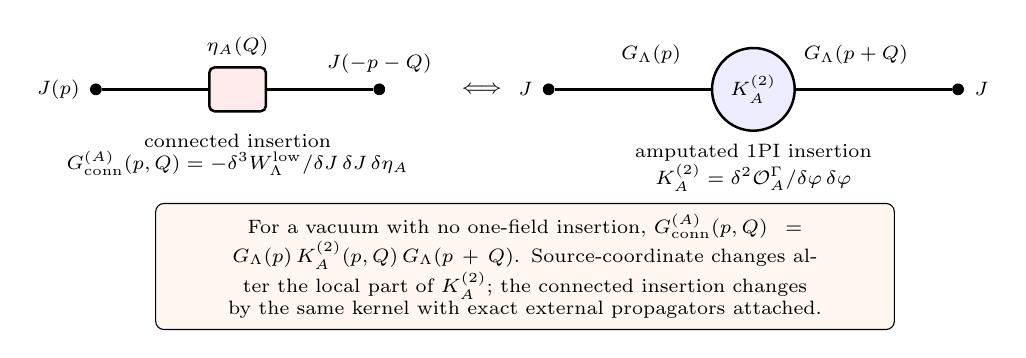
\begin{tikzpicture}[x=1cm,y=1cm,every node/.style={font=\scriptsize}]
    \tikzset{
      ext/.style={circle,fill=black,inner sep=1.5pt},
      kern/.style={draw,circle,line width=0.9pt,minimum size=1.05cm,
        fill=blue!7,align=center},
      op/.style={draw,rectangle,rounded corners=2pt,line width=0.9pt,
        minimum width=0.72cm,minimum height=0.56cm,fill=red!8},
      prop/.style={line width=0.9pt},
      arr/.style={-{Latex[length=2mm]},line width=0.85pt}
    }
    \node[ext,label=left:\(J(p)\)] (l1) at (-4.2,1.05) {};
    \node[ext,label=above:\(J(-p-Q)\)] (r1) at (-0.6,1.05) {};
    \node[op,label=above:\(\eta_A(Q)\)] (cins) at (-2.4,1.05) {};
    \draw[prop] (l1)--(cins)--(r1);
    \node[align=center] at (-2.4,0.22)
      {connected insertion\\
      \(G^{(A)}_{\rm conn}(p,Q)
      =-\delta^3 W_\Lambda^{\rm low}/\delta J\,\delta J\,\delta\eta_A\)};

    \node at (0.70,1.05) {\(\Longleftrightarrow\)};

    \node[ext,label=left:\(J\)] (l2) at (1.55,1.05) {};
    \node[kern] (k) at (4.15,1.05)
      {\(K_A^{(2)}\)};
    \node[ext,label=right:\(J\)] (r2) at (6.75,1.05) {};
    \draw[prop] (l2)--(k)--(r2);
    \node[above] at (2.85,1.24) {\(G_\Lambda(p)\)};
    \node[above] at (5.45,1.24) {\(G_\Lambda(p+Q)\)};
    \node[align=center] at (4.15,0.05)
      {amputated 1PI insertion\\
      \(K_A^{(2)}
       =\delta^2\mathcal O_A^\Gamma/\delta\varphi\,\delta\varphi\)};

    \node[draw,rounded corners=3pt,fill=orange!6,align=center,
      inner sep=4pt,text width=9.1cm] at (1.25,-1.2)
      {For a vacuum with no one-field insertion,
      \(G^{(A)}_{\rm conn}(p,Q)=
      G_\Lambda(p)\,K_A^{(2)}(p,Q)\,G_\Lambda(p+Q)\).
      Source-coordinate changes alter the local part of \(K_A^{(2)}\);
      the connected insertion changes by the same kernel with exact
      external propagators attached.};
  \end{tikzpicture}
  }
  \caption{The Legendre transform changes a connected low-field insertion into
  an amputated 1PI insertion kernel.  In the two-point sector, and when
  one-field insertion terms vanish by the vacuum quantum numbers, the connected
  insertion is obtained by attaching exact low-field propagators to the
  amputated kernel.}
  \label{fig:source-extended-wilsonian-operator-bridge}
\end{figure}

\section{A Worked Insertion: The Mass Operator in \texorpdfstring{\(\phi^4\)}{phi4}}

The abstract source bridge becomes concrete in the scalar quartic theory.
Work at finite regulator in four Euclidean dimensions, and introduce a source
\(\eta\) for the local operator
\[
  O_m(x)=\frac12\phi(x)^2 .
\]
The source-dependent part of the regulated action, in the cutoff-dependent
source coordinate \(\eta_0\), is
\[
  \int\dd^4x\,\eta_0(x)O_m(x).
\]
Let \(Q\) denote the momentum carried by the source insertion, and let
\[
  C_{\Lambda_0}=C_\Lambda+C_>
\]
be the same covariance split used for the Wilsonian action.  For covariances
\(A,B\), define the one-insertion bubble
\[
  \mathcal I_{A,B}(Q)
  =
  \int\frac{\dd^4q}{(2\pi)^4}\,
  A(q)\,B(q+Q).
\]
Then
\begin{equation}
  \mathcal I_{C_{\Lambda_0},C_{\Lambda_0}}(Q)
  =
  \mathcal I_{<,<}(Q)
  +
  \mathcal I_{>,>}(Q)
  +
  \mathcal I_\times(Q),
  \label{eq:operator-insertion-bubble-covariance-split}
\end{equation}
where
\[
  \mathcal I_{<,<}=\mathcal I_{C_\Lambda,C_\Lambda},
  \qquad
  \mathcal I_{>,>}=\mathcal I_{C_>,C_>},
\]
and
\[
  \mathcal I_\times
  =
  \mathcal I_{C_\Lambda,C_>}
  +
  \mathcal I_{C_>,C_\Lambda}.
\]

The Wilsonian insertion functional is the source derivative of
\(L_\Lambda[\phi;\eta_\Lambda]\).  At zeroth order in the quartic coupling,
the Gaussian pushforward gives
\[
  \mathcal O^{\rm W}_{m,\Lambda}(x;\phi)
  =
  \frac12\phi(x)^2
  +
  \frac12 C_>(x,x)
  +
  \cdots ,
\]
where the second term is an identity-operator contribution.  It affects the
vacuum response to \(\eta\), but not the two-field amputated insertion
kernel.  At first order in the quartic coupling \(g\), the coefficient of
\(\frac12\phi^2\) in the Wilsonian insertion receives the high-high bubble:
\begin{equation}
  \mathcal O^{\rm W}_{m,\Lambda}(Q;\phi)
  =
  \left[
    1-\frac{g}{2}\mathcal I_{>,>}(Q)
    +Z^{\rm loc}_{m,\Lambda}(Q)
  \right]
  \frac12(\phi\phi)(Q)
  +
  \hbox{identity and higher local terms}
  +
  O(g^2).
  \label{eq:wilsonian-mass-insertion-one-loop}
\end{equation}
Here \((\phi\phi)(Q)\) denotes the Fourier transform of \(\phi(x)^2\), and
\(Z^{\rm loc}_{m,\Lambda}(Q)\) is the local source-coordinate counterterm and
finite convention.  The factor \(1/2\) is the one-loop symmetry factor in the
normalization \(g\phi^4/4!\) and \(O_m=\phi^2/2\).

Now compare with the BPHZ normal-product definition.  Let
\(\mathcal Q_\mu\) be the nonexceptional source-momentum subtraction
configuration used to define the two-field 1PI insertion kernel, and let
\[
  K_m^{(2)}(Q)
  =
  \frac{\delta^2}{\delta\varphi\,\delta\varphi}
  \mathcal O_m^\Gamma(Q;\varphi)
  \bigg|_{\varphi=0}
\]
in the field normalization of the chosen 1PI coordinate chart.  The
renormalization condition
\[
  K_m^{(2)}(\mathcal Q_\mu)=1
\]
fixes the finite normalization of the renormalized operator.  At one loop,
the BPHZ-subtracted insertion kernel is
\begin{equation}
  K_{m,{\rm BPHZ}}^{(2)}(Q)
  =
  1
  -
  \frac{g}{2}
  \left[
    \mathcal I_{C_{\Lambda_0},C_{\Lambda_0}}(Q)
    -
    \mathcal I_{C_{\Lambda_0},C_{\Lambda_0}}(\mathcal Q_\mu)
  \right]
  +
  O(g^2),
  \label{eq:bphz-mass-insertion-normal-product}
\end{equation}
with the ultraviolet limit taken after the subtraction.  The subtraction is a
local normal-product convention for the operator \(O_m\).
The comparison theorem
Theorem~\ref{thm:finite-order-bphz-wilsonian-matching} treats this finite
normal-product choice as part of the local source-coordinate chart: changing a
Zimmermann normal product changes the finite local operator coordinates and
therefore the source coordinate map.

Figure~\ref{fig:mass-insertion-source-wilsonian-matching} displays the
actual covariance assignment on the one-loop insertion graph.  The loop has
two internal propagator slots; inserting
\(C_{\Lambda_0}=C_\Lambda+C_>\) in each slot gives the low--low,
high--high, and two mixed contributions in
\eqref{eq:operator-insertion-bubble-covariance-split}.

\begin{figure}[H]
  \centering
  \resizebox{0.95\textwidth}{!}{%
  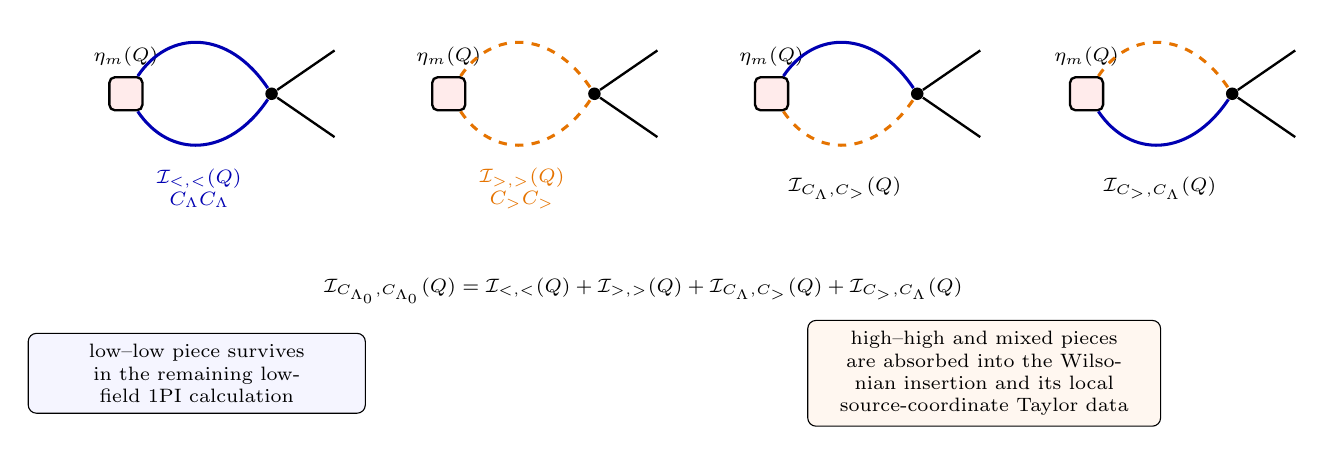
\begin{tikzpicture}[x=1cm,y=1cm,every node/.style={font=\scriptsize}]
    \tikzset{
      ext/.style={circle,fill=black,inner sep=1.35pt},
      op/.style={draw,rectangle,rounded corners=2pt,line width=0.85pt,
        fill=red!8,minimum width=0.42cm,minimum height=0.42cm},
      vtx/.style={circle,fill=black,inner sep=1.6pt},
      low/.style={line width=1.1pt,blue!70!black},
      high/.style={line width=1.1pt,orange!90!black,dashed},
      leg/.style={line width=0.85pt},
      arr/.style={-{Latex[length=2mm]},line width=0.75pt}
    }
    \newcommand{\bubblegraph}[4]{%
      \node[op,label=above:\(\eta_m(Q)\)] (#1o) at (#2,#3) {};
      \node[vtx] (#1v) at (#2+1.85,#3) {};
      \draw[#4] (#1o) .. controls (#2+0.55,#3+0.82) and (#2+1.30,#3+0.82) .. (#1v);
      \draw[#4] (#1o) .. controls (#2+0.55,#3-0.82) and (#2+1.30,#3-0.82) .. (#1v);
      \draw[leg] (#1v)--(#2+2.65,#3+0.55);
      \draw[leg] (#1v)--(#2+2.65,#3-0.55);
    }
    \newcommand{\bubblemix}[5]{%
      \node[op,label=above:\(\eta_m(Q)\)] (#1o) at (#2,#3) {};
      \node[vtx] (#1v) at (#2+1.85,#3) {};
      \draw[#4] (#1o) .. controls (#2+0.55,#3+0.82) and (#2+1.30,#3+0.82) .. (#1v);
      \draw[#5] (#1o) .. controls (#2+0.55,#3-0.82) and (#2+1.30,#3-0.82) .. (#1v);
      \draw[leg] (#1v)--(#2+2.65,#3+0.55);
      \draw[leg] (#1v)--(#2+2.65,#3-0.55);
    }

    \bubblegraph{ll}{-4.95}{1.45}{low}
    \node[align=center,blue!70!black] at (-4.02,0.25)
      {\(\mathcal I_{<,<}(Q)\)\\\(C_\Lambda C_\Lambda\)};

    \bubblegraph{hh}{-0.85}{1.45}{high}
    \node[align=center,orange!90!black] at (0.08,0.25)
      {\(\mathcal I_{>,>}(Q)\)\\\(C_>C_>\)};

    \bubblemix{lh}{3.25}{1.45}{low}{high}
    \node[align=center] at (4.18,0.25)
      {\(\mathcal I_{C_\Lambda,C_>}(Q)\)};

    \bubblemix{hl}{7.25}{1.45}{high}{low}
    \node[align=center] at (8.18,0.25)
      {\(\mathcal I_{C_>,C_\Lambda}(Q)\)};

    \node[align=center] at (1.62,-1.05)
      {\(\mathcal I_{C_{\Lambda_0},C_{\Lambda_0}}(Q)
      =
      \mathcal I_{<,<}(Q)+\mathcal I_{>,>}(Q)
      +\mathcal I_{C_\Lambda,C_>}(Q)+\mathcal I_{C_>,C_\Lambda}(Q)\)};
    \node[draw,rounded corners=3pt,fill=blue!4,align=center,
      inner sep=4pt,text width=4.0cm] at (-4.05,-2.10)
      {low--low piece survives in the remaining low-field 1PI calculation};
    \node[draw,rounded corners=3pt,fill=orange!6,align=center,
      inner sep=4pt,text width=4.2cm] at (5.95,-2.10)
      {high--high and mixed pieces are absorbed into the Wilsonian insertion
      and its local source-coordinate Taylor data};
  \end{tikzpicture}
  }
  \caption{The one-loop mass-operator kernel is a single insertion graph with
  two internal covariance slots.  Expanding
  \(C_{\Lambda_0}=C_\Lambda+C_>\) on those slots gives the four displayed
  assignments; the two mixed assignments form
  \(\mathcal I_\times\).  This is the graph-level content behind the local
  Wilsonian source-coordinate matching.}
  \label{fig:mass-insertion-source-wilsonian-matching}
\end{figure}

The 1PI insertion computed from the Wilsonian description has the form
\begin{equation}
  K_{m,\Lambda}^{(2)}(Q)
  =
  Z_{m,\Lambda}(Q)
  -
  \frac{g}{2}\mathcal I_{<,<}(Q)
  -
  \frac{g}{2}\mathcal I_\times^{\rm loc}(Q)
  +
  O(g^2),
  \label{eq:wilsonian-low-mass-insertion-kernel}
\end{equation}
where \(Z_{m,\Lambda}(Q)\) is the local coefficient multiplying
\(\frac12\phi^2\) in the Wilsonian insertion, and
\(\mathcal I_\times^{\rm loc}\) denotes the Taylor expansion of the mixed
assignment in the chosen low-momentum source chart.  Projecting at
\(\mathcal Q_\mu\) fixes the source-coordinate normalization:
\begin{equation}
  1
  =
  Z_{m,\Lambda}(\mathcal Q_\mu)
  -
  \frac{g}{2}\mathcal I_{<,<}(\mathcal Q_\mu)
  -
  \frac{g}{2}\mathcal I_\times^{\rm loc}(\mathcal Q_\mu)
  +
  O(g^2).
  \label{eq:mass-operator-source-coordinate-normalization}
\end{equation}
Subtracting this condition from
\eqref{eq:wilsonian-low-mass-insertion-kernel} gives the finite insertion
kernel in the 1PI chart:
\[
  K_{m,\Lambda}^{(2)}(Q)
  =
  1
  -
  \frac{g}{2}
  \left[
    \mathcal I_{<,<}(Q)-\mathcal I_{<,<}(\mathcal Q_\mu)
  \right]
  +
  \mathcal T_{\rm high+mix}^{\rm loc}(Q;\mathcal Q_\mu)
  +
  O(g^2).
\]
Here \(\mathcal T_{\rm high+mix}^{\rm loc}(Q;\mathcal Q_\mu)\) is the finite
local Taylor polynomial produced by the high-high and mixed assignments after
the same subtraction condition has been imposed.  Adding this Taylor data
reconstructs the low-momentum expansion of
\eqref{eq:bphz-mass-insertion-normal-product}.  Thus the normal product, the
Wilsonian insertion functional, and the 1PI insertion kernel are distinct
representatives of the same source derivative after the finite-regulator
pushforward, low-field integration, Legendre transform, and source-coordinate
projection have been specified.

This construction also clarifies the transformation law of anomalous
dimensions.  Let \(t=\log\mu\), and suppose a scale-dependent finite
source-coordinate change relates two renormalized operator bases by
\[
  [\widetilde O_A]_\mu
  =
  M_{AI}(\mu)\,[O_I]_\mu .
\]
If
\[
  \frac{\dd}{\dd t}[O_I]_\mu
  =
  -\gamma_{IK}[O_K]_\mu,
\]
then
\[
  \frac{\dd}{\dd t}[\widetilde O_A]_\mu
  =
  -
  \widetilde\gamma_{AB}
  [\widetilde O_B]_\mu
\]
with
\begin{equation}
  \widetilde\gamma
  =
  M\gamma M^{-1}
  -
  \frac{\dd M}{\dd t}M^{-1}.
  \label{eq:operator-anomalous-dimension-connection-law}
\end{equation}

\begin{theorem}[Anomalous dimensions as an RG connection]
\label{thm:anomalous-dimensions-rg-connection}
Let \(\mathcal E\to U\) be a finite-rank renormalized operator bundle on a
coordinate neighborhood \(U\) in theory space.  Assume that the beta-function
vector field \(\beta=\beta_I(g)\partial/\partial g_I\) and the transition
matrices \(M_{\alpha\beta}(g,t)\) between source charts are \(C^1\) along the
RG trajectories under consideration, or are formal power series for which the
following differentiations are performed coefficientwise.  In a local source
chart, let \(e\) denote the local representative column
\(e_I=[O_I]_\mu\), and suppose the RG variation is
\begin{equation}
  \frac{\dd}{\dd t}e_I
  =
  -\gamma_{IK}(g(t),t)e_K .
  \label{eq:operator-frame-parallel-transport}
\end{equation}
Then the matrices \(\gamma\) define a connection on \(\mathcal E\) along the
RG vector field by
\begin{equation}
  (D_t v)_\alpha
  =
  \frac{\dd v_\alpha}{\dd t}+\gamma_\alpha v_\alpha
  \label{eq:operator-bundle-rg-connection}
\end{equation}
for local representative columns \(v_\alpha\) in a source chart \(\alpha\).
Under a finite scale-dependent change of source chart with
\(\widetilde e=M e\) and \(v_{\widetilde\alpha}=M v_\alpha\), the connection
coefficients transform as
\begin{equation}
  \widetilde\gamma
  =
  M\gamma M^{-1}
  -
  \frac{\dd M}{\dd t}M^{-1}.
  \label{eq:operator-connection-transformation-theorem}
\end{equation}
Conversely, any family of matrices obeying
\eqref{eq:operator-connection-transformation-theorem} on overlaps is precisely
the local expression of a connection along the RG vector field.  For the
deformation-operator bundle of Definition~\ref{def:deformation-operator-bundle},
the connection induced by the linearized beta-function flow has
\begin{equation}
  \gamma_{IK}
  =
  \frac{\partial\beta_K}{\partial g_I}
  \label{eq:cotangent-rg-connection-jacobian}
\end{equation}
in the coordinate frame dual to \(g_I\).
\end{theorem}

\begin{proof}
The operator frame equation
\eqref{eq:operator-frame-parallel-transport} is the statement that the chosen
renormalized source-representative column is parallel along the RG trajectory:
\(D_t e=0\) in the local convention of
\eqref{eq:operator-bundle-rg-connection}.  Let \(\widetilde e=M e\).
Differentiating gives
\[
  \frac{\dd}{\dd t}\widetilde e
  =
  \left(\frac{\dd M}{\dd t}M^{-1}-M\gamma M^{-1}\right)\widetilde e .
\]
Writing the same equation in the new chart as
\(\dd\widetilde e/\dd t=-\widetilde\gamma\,\widetilde e\) gives
\eqref{eq:operator-connection-transformation-theorem}.  The same computation
is the patching criterion for a connection along a one-dimensional direction:
if local matrices obey this law, the formula \(D_t v=\dd v/\dd t+\gamma v\)
is independent of the frame because
\[
  \left(\frac{\dd}{\dd t}+\widetilde\gamma\right)\widetilde v
  =
  M\left(\frac{\dd}{\dd t}+\gamma\right)v
  \qquad
  (\widetilde v=Mv).
  \]
Hence the local operators \(D_t\) glue to a well-defined connection along the
RG vector field.

For deformation operators, an infinitesimal tangent vector
\(\delta g_K\partial/\partial g_K\) obeys the variational equation obtained by
linearizing the RG flow:
\[
  \frac{\dd}{\dd t}\delta g_K
  =
  \frac{\partial\beta_K}{\partial g_I}\,\delta g_I .
  \]
The deformation insertion is the pairing
\(\int\delta g_I e_I\).  Bare scale independence of this pairing gives
\[
  0
  =
  \frac{\dd}{\dd t}\bigl(\delta g_I e_I\bigr)
  =
  \frac{\partial\beta_I}{\partial g_K}\delta g_K e_I
  +
  \delta g_I\frac{\dd e_I}{\dd t}.
  \]
Renaming dummy indices and using the arbitrariness of \(\delta g_I\) yields
\[
  \frac{\dd e_I}{\dd t}
  =
  -
  \frac{\partial\beta_K}{\partial g_I}e_K,
  \]
which is \eqref{eq:operator-frame-parallel-transport} with
\(\gamma_{IK}=\partial\beta_K/\partial g_I\).
\end{proof}

Thus the anomalous-dimension matrix transforms by conjugation only for
scale-independent changes of operator coordinates.  For scale-dependent
renormalized source coordinates,
\eqref{eq:operator-anomalous-dimension-connection-law} is the connection
transformation law of Theorem~\ref{thm:anomalous-dimensions-rg-connection}.

\section{Multiple Insertions and Contact-Term Coordinates}
\label{sec:multiple-insertions-contact-coordinates}

The linear source map in
\eqref{eq:source-coordinate-local-differential-map} is the part of the source
coordinate change seen by a single insertion.  Multiple insertions require
the full Taylor expansion of the source chart.  At finite regulator let
\(\mathcal S_\Lambda\) denote the space of regulated source functions
\(\eta_\Lambda^A(x)\).  A local source coordinate chart is a smooth map
\[
  \mathcal Z_\Lambda:\mathcal S_\Lambda\longrightarrow \mathcal S_0,
  \qquad
  \eta_0=\mathcal Z_\Lambda(\eta_\Lambda),
\]
whose Taylor coefficients at the origin are local distributions.  Explicitly,
\begin{equation}
  \eta_0^I(z)
  =
  \sum_{r\ge1}\frac1{r!}
  \int\prod_{a=1}^r\dd^D x_a\,
  \mathcal Z^I{}_{A_1\cdots A_r}
    (z;x_1,\ldots,x_r)
  \eta_\Lambda^{A_1}(x_1)\cdots\eta_\Lambda^{A_r}(x_r).
  \label{eq:local-source-coordinate-taylor-map}
\end{equation}
The \(r=1\) coefficient is the linear differential operator in
\eqref{eq:source-coordinate-local-differential-map}.  For \(r\ge2\), locality
means that
\(\mathcal Z^I{}_{A_1\cdots A_r}(z;x_1,\ldots,x_r)\) is supported on the
small diagonal \(z=x_1=\cdots=x_r\) and is a finite sum of derivatives of
delta functions, with coefficients depending on the chosen regulator scale
and subtraction convention.  These higher Taylor coefficients do not
contribute for separated insertion points, but they determine the extension
of inserted correlators as distributions across collision diagonals.

Let
\[
  G^0_{I_1\cdots I_s}(z_1,\ldots,z_s;J)
  =
  (-1)^s
  \frac{\delta^s W_{\Lambda_0}[J,\eta_0]}
       {\delta\eta_0^{I_1}(z_1)\cdots
        \delta\eta_0^{I_s}(z_s)}
  \bigg|_{\eta_0=0}
\]
be the connected bare distribution with \(s\) operator insertions and
arbitrary external source \(J\).  The renormalized distribution in the source
coordinate \(\eta_\Lambda\) is
\[
  G^\Lambda_{A_1\cdots A_r}(x_1,\ldots,x_r;J)
  =
  (-1)^r
  \frac{\delta^r W_{\Lambda_0}[J,\mathcal Z_\Lambda(\eta_\Lambda)]}
       {\delta\eta_\Lambda^{A_1}(x_1)\cdots
        \delta\eta_\Lambda^{A_r}(x_r)}
  \bigg|_{\eta_\Lambda=0}.
\]
Set
\[
  H[\eta_\Lambda]=
  W_{\Lambda_0}[J,\mathcal Z_\Lambda(\eta_\Lambda)] .
\]
The functional Fa\`a di Bruno formula for this composite map gives, before
rewriting functional derivatives as insertion distributions,
\[
  \left.
  \frac{\delta^r H}
       {\delta\eta_\Lambda^{A_1}(x_1)\cdots
        \delta\eta_\Lambda^{A_r}(x_r)}
  \right|_{\eta_\Lambda=0}
  =
  \sum_{\pi\in\mathrm{Part}(r)}
  \int\prod_{B\in\pi}\dd^D z_B\,
  \left.
  \frac{\delta^{|\pi|}W_{\Lambda_0}[J,\eta_0]}
       {\prod_{B\in\pi}\delta\eta_0^{I_B}(z_B)}
  \right|_{\eta_0=0}
  \prod_{B\in\pi}
  \mathcal Z^{I_B}{}_{A_B}
    (z_B;x_B).
\]
The partition records which of the \(r\) renormalized source derivatives hit
the same Taylor coefficient of the nonlinear source map
\(\mathcal Z_\Lambda\).  The signs in the final partition formula are not
additional signs attached to the Taylor coefficients of \(\mathcal Z_\Lambda\).
They come from rewriting the ordinary Fa\`a di Bruno identity for the connected
functional \(W=\log Z\) in terms of connected insertion derivatives.  Define
\[
  D^\Lambda_A:=-\frac{\delta}{\delta\eta_\Lambda^A},
  \qquad
  D^0_I:=-\frac{\delta}{\delta\eta_0^I}.
\]
Then \(G^\Lambda_{A_1\cdots A_r}=D^\Lambda_{A_1}\cdots
D^\Lambda_{A_r}H|_{\eta_\Lambda=0}\), while
\(G^0_{I_1\cdots I_s}=D^0_{I_1}\cdots D^0_{I_s}
W_{\Lambda_0}|_{\eta_0=0}\).  Because the displayed Fa\`a di Bruno formula was
written with ordinary derivatives \(\delta/\delta\eta\), the left side obeys
\[
  \begin{aligned}
  G^\Lambda_{A_1\cdots A_r}(x_1,\ldots,x_r;J)
  &=
  (-1)^r
  \left.
  \frac{\delta^r H}
       {\delta\eta_\Lambda^{A_1}(x_1)\cdots
        \delta\eta_\Lambda^{A_r}(x_r)}
  \right|_{\eta_\Lambda=0}.
  \end{aligned}
\]
For the bare connected cumulant attached to a partition \(\pi\),
\[
  \begin{aligned}
  \left.
  \frac{\delta^{|\pi|}W_{\Lambda_0}[J,\eta_0]}
       {\prod_{B\in\pi}\delta\eta_0^{I_B}(z_B)}
  \right|_{\eta_0=0}
  &=
  (-1)^{|\pi|}
  G^0_{I_B\,:\,B\in\pi}(z_B\,:\,B\in\pi;J).
  \end{aligned}
\]
Thus a term indexed by \(\pi\) carries the chain-rule cumulant factor
\[
  (-1)^r(-1)^{|\pi|}
  =
  (-1)^{r-|\pi|}.
\]
Equivalently, a block \(B\) of size \(|B|\) collapses \(|B|\) renormalized
insertion derivatives into one bare connected cumulant and contributes the
relative sign \((-1)^{|B|-1}\); multiplying over the blocks gives
\((-1)^{\sum_B(|B|-1)}=(-1)^{r-|\pi|}\).  The finite-regulator partition
formula is therefore
\begin{equation}
  \begin{aligned}
  G^\Lambda_{A_1\cdots A_r}(x_1,\ldots,x_r;J)
  &=
  \sum_{\pi\in\mathrm{Part}(r)}
  (-1)^{r-|\pi|}
  \int\prod_{B\in\pi}\dd^D z_B\,
  G^0_{I_B\,:\,B\in\pi}(z_B\,:\,B\in\pi;J)
  \\
  &\hspace{2.0cm}\times
  \prod_{B\in\pi}
  \mathcal Z^{I_B}{}_{A_B}
    (z_B;x_B).
  \end{aligned}
  \label{eq:multi-insertion-source-partition-formula}
\end{equation}
Here \(\mathrm{Part}(r)\) is the set of partitions of
\(\{1,\ldots,r\}\).  If \(B=\{b_1,\ldots,b_s\}\), then
\[
  \mathcal Z^{I_B}{}_{A_B}(z_B;x_B)
  =
  \mathcal Z^{I_B}{}_{A_{b_1}\cdots A_{b_s}}
    (z_B;x_{b_1},\ldots,x_{b_s}).
\]

For two insertions the formula reads
\begin{equation}
  \begin{aligned}
  G^\Lambda_{AB}(x,y;J)
  &=
  \int\dd^D z\,\dd^D w\,
  \mathcal Z^I{}_A(z;x)\mathcal Z^J{}_B(w;y)
  G^0_{IJ}(z,w;J)
  \\
  &\quad
  -
  \int\dd^D z\,
  \mathcal Z^I{}_{AB}(z;x,y)
  G^0_I(z;J).
  \end{aligned}
  \label{eq:two-insertion-contact-coordinate-formula}
\end{equation}
The first term is the product of the single-insertion linear maps.  The
second term is supported at \(x=y\) and is therefore a contact term.

On the configuration space
\[
  \mathrm{Conf}_r
  =
  \{(x_1,\ldots,x_r)\mid x_a\ne x_b\ {\rm for}\ a\ne b\},
\]
only the partition of \(\{1,\ldots,r\}\) into singletons contributes to
\eqref{eq:multi-insertion-source-partition-formula}.  All other partitions
are local distributions supported on collision diagonals.
If a block \(B\) has more than one element, the corresponding Taylor
coefficient
\[
  \mathcal Z^{I_B}{}_{A_B}(z_B;x_B)
\]
is supported on the diagonal where all points \(x_b\), \(b\in B\), coincide
with \(z_B\).  This support does not intersect \(\mathrm{Conf}_r\).  The only
surviving term away from the collision diagonals is therefore the singleton
partition, for which every Taylor coefficient is the linear source map.

The same structure appears directly in the Wilsonian representation.  Define
higher Wilsonian source derivatives by
\[
  \mathcal O^{\rm W}_{A_1\cdots A_r}(x_1,\ldots,x_r;\phi)
  =
  \frac{\delta^r L_\Lambda[\phi;\eta_\Lambda]}
       {\delta\eta_\Lambda^{A_1}(x_1)\cdots
        \delta\eta_\Lambda^{A_r}(x_r)}
  \bigg|_{\eta_\Lambda=0}.
\]
For two insertions, differentiating the low-field functional integral gives
\begin{equation}
  G^\Lambda_{AB}(x,y;J)
  =
  \bigl\langle
    \mathcal O^{\rm W}_A(x)\mathcal O^{\rm W}_B(y)
  \bigr\rangle_{\!{\rm conn},J,\Lambda}^{\rm low}
  -
  \bigl\langle
    \mathcal O^{\rm W}_{AB}(x,y)
  \bigr\rangle_{J,\Lambda}^{\rm low}.
  \label{eq:wilsonian-two-insertion-contact-term}
\end{equation}
Thus the contact term is the second source derivative of the
source-extended Wilsonian action in the chosen source chart.

For 1PI coordinates one must also distinguish the source Hessian of the
Legendre transform from the connected two-insertion distribution.  In
condensed notation, with field indices \(i,j\) integrated or summed,
\[
  \left.\frac{\delta^2\Gamma_\Lambda}
    {\delta\eta_\Lambda^A\delta\eta_\Lambda^B}\right|_\varphi
  =
  \left.\frac{\delta^2 W_\Lambda^{\rm low}}
    {\delta\eta_\Lambda^A\delta\eta_\Lambda^B}\right|_J
  -
  \frac{\delta^2 W_\Lambda^{\rm low}}
       {\delta\eta_\Lambda^A\delta J_i}
  \left(
    \frac{\delta^2 W_\Lambda^{\rm low}}
         {\delta J_i\delta J_j}
  \right)^{-1}
  \frac{\delta^2 W_\Lambda^{\rm low}}
       {\delta J_j\delta\eta_\Lambda^B}.
\]
This is the finite-dimensional Legendre-transform identity applied to the
regulated theory.  The second term subtracts the part connected by one
low-field two-point function.  Consequently projected 1PI multi-insertion
kernels have a contact-term convention inherited from both the nonlinear
source chart and the Legendre-transform projection.

Figure~\ref{fig:multi-insertion-contact-source-jets} records the geometric
support statement behind contact terms.  The linear jet acts on the open
configuration space of separated points.  Higher source jets are local
distributions supported on pairwise and higher collision diagonals, and the
Legendre transform adds the separate one-low-field-reducible subtraction
displayed above.

\begin{figure}[H]
  \centering
  \resizebox{0.90\textwidth}{!}{%
  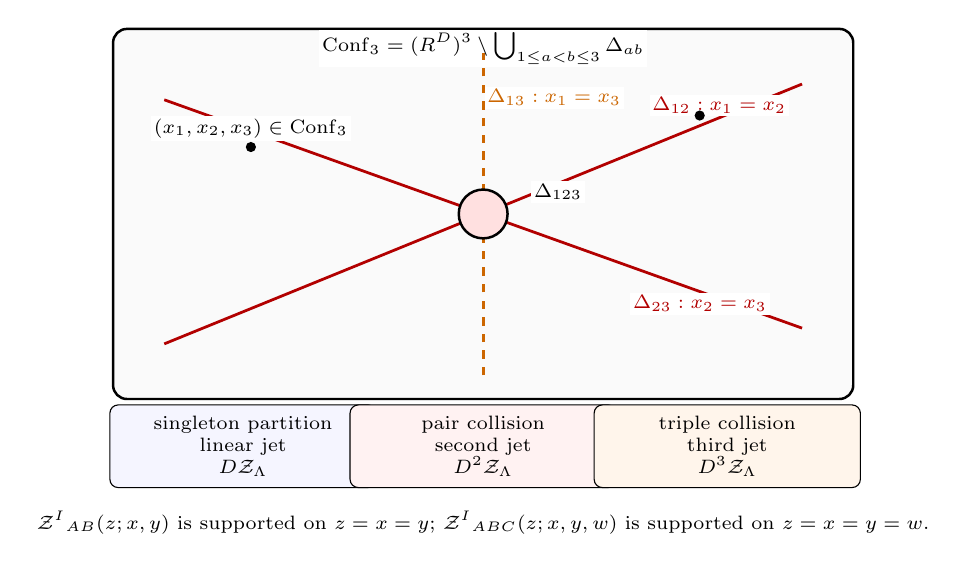
\begin{tikzpicture}[x=1cm,y=1cm,every node/.style={font=\scriptsize}]
    \tikzset{
      diag/.style={line width=1.0pt,red!70!black},
      pdiag/.style={line width=1.0pt,orange!80!black,dashed},
      pt/.style={circle,fill=black,inner sep=1.3pt},
      note/.style={draw,rounded corners=3pt,fill=blue!4,align=center,
        inner sep=4pt,text width=3.1cm}
    }
    \draw[rounded corners=5pt,line width=0.9pt,fill=gray!4]
      (-4.7,-2.35) rectangle (4.7,2.35);
    \node[fill=white,inner sep=1pt] at (0,2.10)
      {\(\mathrm{Conf}_3=(\mathbb R^D)^3\setminus
      \bigcup_{1\le a<b\le 3}\Delta_{ab}\)};

    \draw[diag] (-4.05,-1.65)--(4.05,1.65)
      node[pos=0.87,above,fill=white,inner sep=1pt] {\(\Delta_{12}:x_1=x_2\)};
    \draw[diag] (-4.05,1.45)--(4.05,-1.45)
      node[pos=0.84,below,fill=white,inner sep=1pt] {\(\Delta_{23}:x_2=x_3\)};
    \draw[pdiag] (0,-2.05)--(0,2.05)
      node[pos=0.86,right,fill=white,inner sep=1pt] {\(\Delta_{13}:x_1=x_3\)};
    \node[draw,circle,fill=red!12,line width=0.9pt,minimum size=0.62cm]
      (triple) at (0,0) {};
    \node[fill=white,inner sep=1pt] at (0.95,0.28)
      {\(\Delta_{123}\)};

    \node[pt] (confpt) at (-2.95,0.85) {};
    \node[above,fill=white,inner sep=1pt] at (confpt.north)
      {\((x_1,x_2,x_3)\in\mathrm{Conf}_3\)};
    \node[pt] at (2.75,1.25) {};
    \node[note] at (-3.05,-2.95)
      {singleton partition\\linear jet\\\(D\mathcal Z_\Lambda\)};
    \node[note,fill=red!5] at (0,-2.95)
      {pair collision\\second jet\\\(D^2\mathcal Z_\Lambda\)};
    \node[note,fill=orange!8] at (3.10,-2.95)
      {triple collision\\third jet\\\(D^3\mathcal Z_\Lambda\)};

    \node[align=center] at (0,-3.92)
      {\(\mathcal Z^I{}_{AB}(z;x,y)\) is supported on \(z=x=y\);
      \(\mathcal Z^I{}_{ABC}(z;x,y,w)\) is supported on
      \(z=x=y=w\).};
  \end{tikzpicture}
  }
  \caption{Contact terms are support statements on configuration space.  The
  singleton part of the source Taylor expansion acts on separated insertion
  points; higher Taylor coefficients are local distributions on collision
  strata, such as the pairwise diagonals \(\Delta_{ab}\) and the triple
  diagonal \(\Delta_{123}\) for three insertions.}
  \label{fig:multi-insertion-contact-source-jets}
\end{figure}

\section{Anomalous Dimensions and Scaling Operators}

If a basis can be chosen along the flow in which
\[
  \gamma_{IK}(g(\mu))=\delta_{IK}\gamma_I(g(\mu)),
\]
then the operator equation integrates to
\[
  [O_I]_\mu
  =
  \exp\!\left[
    -\int_{\mu'}^\mu
    \frac{\dd\widetilde\mu}{\widetilde\mu}\,
    \gamma_I(g(\widetilde\mu))
  \right]
  [O_I]_{\mu'} .
\]
At an RG fixed point, \(g(\mu)=g_\ast\), the entries \(\gamma_I(g_\ast)\) are
constant.  The anomalous part of the scaling is then
\[
  [O_I]_\mu
  =
  \left(\frac{\mu}{\mu'}\right)^{-\gamma_I}
  [O_I]_{\mu'} .
\]
An operator basis that diagonalizes \(\gamma\) at the fixed point is a basis of
scaling operators for the anomalous part of dilatations.  The full scaling
dimension also includes the engineering dimension assigned before
renormalization.

The elementary field is the simplest special case.  Consider the deformation
\[
  \delta S=\int\dd^Dx\,\delta g_1\,\phi(x).
\]
The amputated 1PI insertion is the external field insertion with the same
normalization already used in the propagator.  Hence
\[
  \delta g_1(\mu)=Z(\mu)^{1/2}\delta g_1,
  \qquad
  [\phi]_\mu=Z(\mu)^{-1/2}\phi .
\]
The field anomalous dimension in this convention is
\[
  \gamma_\phi
  =
  -\frac{\dd\log Z(\mu)^{-1/2}}{\dd\log\mu}
  =
  \frac12\frac{\dd\log Z(\mu)}{\dd\log\mu}.
\]
At a fixed point, constant \(\gamma_\phi\) gives
\[
  Z(\mu)\propto \mu^{2\gamma_\phi}.
\]

\section{Callan--Symanzik Equations With Operator Insertions}

The operator mixing equation gives the insertion version of the
Callan--Symanzik equation.  Let
\[
  G_{0,J,\Lambda}^{(n)}
  (x;x_1,\ldots,x_n;g_0,\Lambda)
  =
  \left\langle
    O_J(x)\,\phi_0(x_1)\cdots\phi_0(x_n)
  \right\rangle_{\!{\rm conn},\Lambda,g_0}
\]
be the regulated bare connected correlator with one bare operator insertion.
Let \(G_I^{(n)}\) denote the corresponding renormalized correlator with one
insertion of \([O_I]_\mu\) and \(n\) elementary renormalized fields:
\[
  G_I^{(n)}
  =
  \left\langle
    [O_I]_\mu(x)\,
    \phi_R(x_1)\cdots\phi_R(x_n)
  \right\rangle_{\rm conn}.
\]
Away from coincident points, the renormalization chart gives
\[
  G_I^{(n)}
  =
  Z_\phi^{-n/2}\,N_{IJ}\,G_{0,J,\Lambda}^{(n)}
\]
after the cutoff-removal limit.  Repeated bare-operator labels are summed.

\begin{proposition}[Insertion Callan--Symanzik equation]
For noncoincident points \(x,x_1,\ldots,x_n\), the renormalized insertion
correlators satisfy
\begin{equation}
  \left(
    \mu\frac{\partial}{\partial\mu}
    +
    \beta_A(g)\frac{\partial}{\partial g_A}
    +
    n\gamma_\phi(g)
  \right)G_I^{(n)}
  +
  \gamma_{IK}(g)G_K^{(n)}
  =
  0 .
  \label{eq:cs-with-operator-mixing}
\end{equation}
\end{proposition}

\begin{proof}
Let \(t=\log\mu\).  The bare correlator
\(G_{0,J,\Lambda}^{(n)}\) has no independent dependence on \(t\) at fixed bare
couplings and cutoff.  Differentiating
\[
  G_I^{(n)}
  =
  Z_\phi^{-n/2}N_{IJ}G_{0,J,\Lambda}^{(n)}
\]
at fixed bare data gives
\[
  \left(
    \frac{\partial}{\partial t}
    +
    \beta_A\frac{\partial}{\partial g_A}
  \right)G_I^{(n)}
  =
  -n\gamma_\phi\,G_I^{(n)}
  +
  \frac{\dd N_{IJ}}{\dd t}\,
  Z_\phi^{-n/2}G_{0,J,\Lambda}^{(n)} .
\]
Using
\[
  \frac{\dd N_{IJ}}{\dd t}
  =
  -\gamma_{IK}N_{KJ}
\]
turns the last term into \(-\gamma_{IK}G_K^{(n)}\).  Moving both
renormalization-factor contributions to the left gives
\eqref{eq:cs-with-operator-mixing}.
\end{proof}

Contact terms must be added when \(x\) collides with one of the other
insertion points, or when several inserted operators are present and collide
with one another.  Those terms are local distributions supported on collision
diagonals, as described by the source-coordinate Taylor expansion in
Section~\ref{sec:multiple-insertions-contact-coordinates}.  Their coefficients
are governed by the same renormalized local operator basis, but they depend on
the contact-term convention chosen for the source-renormalized generating
functional.

At a fixed point, diagonalizing \(\gamma_{IK}(g_\ast)\) gives scaling
operators.  If \([O_A]\) is an eigenoperator with anomalous dimension
\(\gamma_A\), then its full scaling dimension is
\[
  \Delta_A=d_A+\gamma_A,
\]
where \(d_A\) is the engineering dimension in the fixed-point convention.
Equation \eqref{eq:cs-with-operator-mixing} is then the differential form of
homogeneous scaling of correlation functions with an \(O_A\) insertion.

\section{Dimensional Regularization and MS Coordinates}

Now formulate the same 1PI RG in dimensional regularization.  Let
\[
  D=d-\epsilon
\]
and write the Euclidean action as
\[
  S[\phi]
  =
  S_{\rm kin}[\phi]
  +
  \int\dd^{d-\epsilon}x\,
  \sum_I g_I^\epsilon\,O_I(x).
\]
The superscript on \(g_I^\epsilon\) records dependence on the regulator
\(\epsilon\).  The engineering dimensions are assigned as
\[
  [\phi]=\frac{d-\epsilon-2}{2},
  \qquad
  [O_I]=d-\epsilon+\delta_I(\epsilon),
  \qquad
  [g_I^\epsilon]=-\delta_I(\epsilon),
\]
where
\[
  \delta_I(\epsilon)=\delta_I^{(0)}+\epsilon\,\delta_I^{(1)}.
\]

\begin{definition}[Minimal subtraction coordinates]
The minimal-subtraction coordinate \(\lambda_I(\mu)\) is defined by the
requirement that the bare coupling have the form
\[
  g_I^\epsilon
  =
  \mu^{-\delta_I(\epsilon)}
  \left[
    \lambda_I(\mu)
    +
    \sum_{n\ge1}
    \frac{1}{\epsilon^n}
    K_I^{(n)}(\lambda(\mu))
  \right].
\]
The functions \(K_I^{(n)}\) are formal power series in the dimensionless
coordinates \(\lambda_J\).  The bracket contains the finite coordinate
\(\lambda_I\) and pole terms in \(\epsilon\); finite terms in the counterterm
part are set to zero by the MS coordinate convention.
\end{definition}

The MS convention fixes the finite redefinition freedom present in a general
subtraction coordinate.  It is especially convenient because the beta functions
and anomalous dimensions are encoded in the pole coefficients.

Figure~\ref{fig:volume-ii-ms-coordinate-structure} depicts the MS coordinate
as a Laurent-principal-part prescription at \(\epsilon=0\).  The finite
coordinate \(\lambda_I\) is the regular part selected after the pole part has
been subtracted; the pole coefficients \(K_I^{(n)}\) are the residues of the
principal part in this formal meromorphic coordinate.

\begin{figure}[H]
  \centering
  \resizebox{0.88\textwidth}{!}{%
  \begin{tikzpicture}[x=1cm,y=1cm,every node/.style={font=\scriptsize}]
    \tikzset{
      pole/.style={line width=0.8pt,red!70!black},
      arr/.style={-{Latex[length=2mm]},line width=0.85pt}
    }
    \draw[->] (-3.8,0)--(3.8,0) node[right] {\(\operatorname{Re}\epsilon\)};
    \draw[->] (0,-2.05)--(0,2.05) node[above] {\(\operatorname{Im}\epsilon\)};
    \draw[line width=0.9pt,blue!65!black] (0,0) circle (0.58);
    \fill[red!70!black] (0,0) circle (1.8pt);
    \node[above right] at (0.08,0.08) {\(\epsilon=0\)};
    \draw[pole] (-0.15,-1.45)--(0.15,1.45);
    \draw[pole] (-0.32,-1.18)--(0.32,1.18);
    \node[red!70!black,align=center] at (-2.35,1.30)
      {principal part\\
      \(\sum_{n\ge1}\epsilon^{-n}K_I^{(n)}(\lambda)\)};
    \draw[arr,red!70!black] (-1.35,1.05)--(-0.28,0.40);
    \node[blue!65!black,align=center] at (2.45,1.12)
      {regular part\\\(\lambda_I(\mu)\)};
    \draw[arr,blue!65!black] (1.56,0.95)--(0.48,0.25);
    \node[draw,rounded corners=3pt,fill=gray!4,align=center,
      inner sep=5pt,text width=8.9cm] at (0,-2.95)
      {\(\displaystyle
        g_I^\epsilon=\mu^{-\delta_I(\epsilon)}
        \left[
        \lambda_I(\mu)+
        \underbrace{\sum_{n\ge1}\epsilon^{-n}K_I^{(n)}(\lambda(\mu))}_{P_-
        \text{ principal part}}
        \right],
        \quad
        P_{\rm fin}\bigl(\mu^{\delta_I(\epsilon)}g_I^\epsilon\bigr)
        =\lambda_I .
      \)};
  \end{tikzpicture}
  }
  \caption[Minimal-subtraction coordinate and pole data]{Minimal subtraction
  is a Laurent projection at the regulator point \(\epsilon=0\).  The
  dimensionless running coordinate is the finite part after the principal
  pole part has been subtracted.  The coefficients \(K_I^{(n)}\) are then
  constrained by the condition
  \(\dd g_I^\epsilon/\dd\log\mu=0\).}
  \label{fig:volume-ii-ms-coordinate-structure}
\end{figure}

\section{The Scalar Quartic Pole at One Loop}
\label{sec:volume-ii-scalar-quartic-pole-one-loop}

For \(d=4\), consider the scalar quartic operator with dimensional
regularization \(D=4-\epsilon\).  The quartic coupling \(g^\epsilon\) has
engineering dimension \(\epsilon\), and the interaction term is
\[
  \mathcal L_E\supset \frac1{4!}g^\epsilon\phi^4 .
\]
A general momentum-subtraction coordinate
\(\widetilde\lambda(\mu)\) can be defined at Euclidean momenta of size
\(\mu\):
\[
  \mu^\epsilon \widetilde\lambda(\mu)
  =
  -Z(\mu)^2\,
  \Gamma^{(4)}
  \bigg|_{k_i^2=O(\mu^2),\;
  s=-\mu^2a_s,\;t=-\mu^2a_t,\;u=-\mu^2a_u},
\]
where \(a_s,a_t,a_u>0\) are fixed constants specifying the subtraction
configuration.

At one loop,
\[
\begin{aligned}
  \mu^\epsilon\widetilde\lambda(\mu)
  &=
  g^\epsilon
  -
  \frac{(g^\epsilon)^2}{2}
  \int\frac{\dd^{4-\epsilon}k}{(2\pi)^{4-\epsilon}}
  \int_0^1\dd x                                      \\
  &\quad\times
  \left[
    \frac{1}{(k^2+\mu^2a_sx(1-x))^2}
    +(a_s\to a_t)+(a_s\to a_u)
  \right]
  +
  O((g^\epsilon)^3).
\end{aligned}
\]
Using
\[
  \int\frac{\dd^{4-\epsilon}k}{(2\pi)^{4-\epsilon}}
  \frac{1}{(k^2+\Delta)^2}
  =
  (4\pi)^{-2+\epsilon/2}
  \Gamma\!\left(\frac{\epsilon}{2}\right)
  \Delta^{-\epsilon/2},
\]
and then integrating over \(x\), this becomes
\[
\begin{aligned}
  \mu^\epsilon\widetilde\lambda(\mu)
  &=
  g^\epsilon
  -
  \frac{(g^\epsilon)^2}{2}\,
  \mu^{-\epsilon}
  (4\pi)^{-2+\epsilon/2}
  \frac{\Gamma(\epsilon/2)\Gamma(1-\epsilon/2)^2}
       {\Gamma(2-\epsilon)}
       \\
  &\quad\times
  \left(
    a_s^{-\epsilon/2}
    +a_t^{-\epsilon/2}
    +a_u^{-\epsilon/2}
  \right)
  +
  O((g^\epsilon)^3).
\end{aligned}
\]
Inverting the relation gives
\[
  g^\epsilon
  =
  \mu^\epsilon
  \left[
    \widetilde\lambda(\mu)
    +
    \widetilde\lambda(\mu)^2
    \left(
      \frac{3}{16\pi^2}\frac1{\epsilon}
      +
      O(\epsilon^0)
    \right)
    +
    O(\widetilde\lambda^3)
  \right].
\]
The \(O(\epsilon^0)\) term depends on the finite subtraction constants
\(a_s,a_t,a_u\).  The MS coordinate \(\lambda(\mu)\) is defined by retaining
the pole coefficient and setting the finite counterterm convention to zero:
\[
  g^\epsilon
  =
  \mu^\epsilon
  \left[
    \lambda(\mu)
    +
    \frac{3}{16\pi^2}
    \frac{\lambda(\mu)^2}{\epsilon}
    +
    O(\lambda^3)
  \right].
\]
This equation fixes the notation used later.  For the Wilson--Fisher
calculation, the bare quartic coefficient \(g_0\) is this \(g^\epsilon\), and
the dimensionful running quartic coefficient is
\[
  g_R(\mu)=\mu^\epsilon\lambda(\mu).
\]
For Yang--Mills theory the coupling is placed in the inverse kinetic
coefficient, so the analogous dimensionless coordinate is written
\[
  \lambda_{\rm YM}^2(\mu)=\mu^\epsilon g_{\rm YM}^2(\mu),
  \qquad
  \frac1{g_{\rm YM}^2(\mu)}
  =
  \mu^\epsilon\frac1{\lambda_{\rm YM}^2(\mu)} .
\]
Thus the power of \(\mu\) is the same engineering-dimension conversion; only
the choice of coupling coordinate differs between a polynomial scalar vertex
and an inverse gauge kinetic term.

Figure~\ref{fig:volume-ii-phi-four-ms-pole} displays the one-loop quartic MS
structure in this convention: the logarithmic scalar bubble supplies the pole
subtraction, and the engineering power of \(\mu\) converts the coordinate in
\(4-\epsilon\) dimensions.

\begin{figure}[H]
  \centering
  \resizebox{0.88\textwidth}{!}{%
  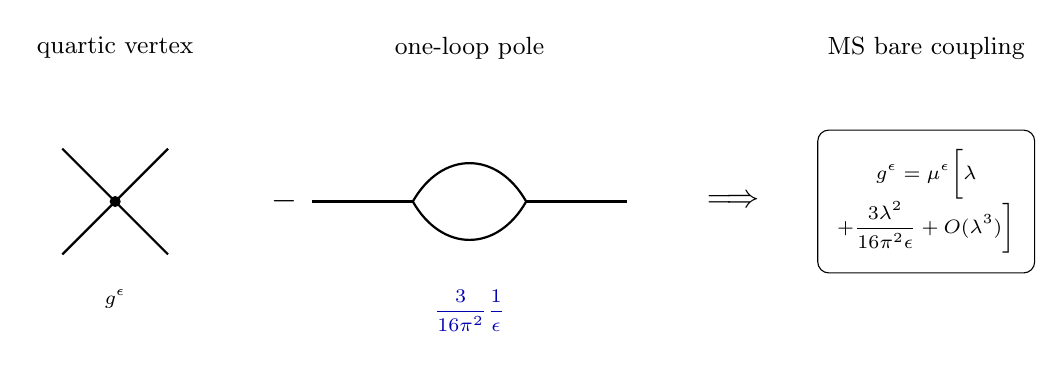
\begin{tikzpicture}[x=1cm,y=1cm,every node/.style={font=\scriptsize}]
    \begin{scope}
      \node[font=\small] at (0,1.95) {quartic vertex};
      \foreach \a in {45,135,225,315} {
        \draw[thick] (0,0)--++({0.95*cos(\a)},{0.95*sin(\a)});
      }
      \fill[black] (0,0) circle (2pt);
      \node[below] at (0,-1.0) {\(g^\epsilon\)};
    \end{scope}

    \node[font=\large] at (2.15,0) {\(-\)};

    \begin{scope}[shift={(4.5,0)}]
      \node[font=\small] at (0,1.95) {one-loop pole};
      \draw[thick] (-2.0,0)--(-0.72,0);
      \draw[thick] (0.72,0)--(2.0,0);
      \draw[thick] (-0.72,0)..controls (-0.35,0.65) and (0.35,0.65)..(0.72,0);
      \draw[thick] (-0.72,0)..controls (-0.35,-0.65) and (0.35,-0.65)..(0.72,0);
      \node[blue!70!black, below] at (0,-1.0)
        {\(\displaystyle \frac{3}{16\pi^2}\frac1{\epsilon}\)};
    \end{scope}

    \node[font=\large] at (7.85,0) {\(\Longrightarrow\)};

    \begin{scope}[shift={(10.3,0)}]
      \node[font=\small] at (0,1.95) {MS bare coupling};
      \node[draw=black, rounded corners, align=center, inner sep=7pt] at (0,0)
        {\(g^\epsilon=\mu^\epsilon\bigl[\lambda\)\\
         \(\displaystyle +\frac{3\lambda^2}{16\pi^2\epsilon}
         +O(\lambda^3)\bigr]\)};
    \end{scope}
  \end{tikzpicture}
  }
  \caption{In four-dimensional scalar quartic theory, the one-loop bubble
  produces the pole coefficient \(3/(16\pi^2\epsilon)\).  The MS coordinate
  keeps this pole coefficient in the bare coupling and fixes the finite part
  by convention.}
  \label{fig:volume-ii-phi-four-ms-pole}
\end{figure}

\section{Beta Functions Away from the Target Dimension}

In MS coordinates define
\[
  \beta_I^\epsilon(\lambda)
  =
  \frac{\dd\lambda_I(\mu)}{\dd\log\mu}.
\]
The bare coupling \(g_I^\epsilon\) is independent of \(\mu\).  Differentiating
the MS definition gives
\[
\begin{aligned}
  0
  &=
  \frac{\dd g_I^\epsilon}{\dd\log\mu}                         \\
  &=
  -\delta_I(\epsilon)
  \left[
    \lambda_I+\sum_{n\ge1}\epsilon^{-n}K_I^{(n)}
  \right]
  +
  \beta_I^\epsilon
  +
  \sum_{n\ge1}\epsilon^{-n}
  \frac{\partial K_I^{(n)}}{\partial\lambda_J}
  \beta_J^\epsilon .
\end{aligned}
\]
Here and below repeated \(J\)-indices are summed.  Expand the
\((d-\epsilon)\)-dimensional beta function as
\[
  \beta_I^\epsilon(\lambda)
  =
  \sum_{m=0}^\infty
  \epsilon^m\beta_I^{(m)}(\lambda).
\]
The positive powers of \(\epsilon\) are constrained by the displayed equation.
For example, the coefficient of \(\epsilon^1\) has the form
\[
  -\delta_I^{(1)}\lambda_I
  +
  \beta_I^{(1)}
  +
  \sum_{n\ge1}
  \frac{\partial K_I^{(n)}}{\partial\lambda_J}
  \beta_J^{(n+1)}
  =
  0,
\]
and the coefficient of \(\epsilon^2\) has the form
\[
  \beta_I^{(2)}
  +
  \sum_{n\ge1}
  \frac{\partial K_I^{(n)}}{\partial\lambda_J}
  \beta_J^{(n+2)}
  =
  0.
\]
The pole \(K_I^{(n)}\) begins at increasingly high perturbative order as
\(n\) grows.  More precisely, grade the formal power series by perturbative
degree and assume \(K_I^{(n)}\in F^{n+1}\), where \(F^L\) denotes terms of
degree at least \(L\) in the interaction coordinates.  Then
\(\partial K_I^{(n)}/\partial\lambda_J\in F^n\).  For the coefficient of
\(\epsilon^r\) with \(r\ge2\), the homogeneous degree-\(L\) part of
\[
  \beta_I^{(r)}
  +
  \sum_{n\ge1}
  \frac{\partial K_I^{(n)}}{\partial\lambda_J}
  \beta_J^{(n+r)}
  =
  0
\]
contains \(\beta_J^{(n+r)}\) only in degrees strictly smaller than \(L\).
Writing \(\beta_{I,L}^{(r)}\) for the degree-\(L\) component, the lowest
perturbative degree therefore gives \(\beta_{I,L}^{(r)}=0\), and induction on
\(L\) gives \(\beta_I^{(r)}=0\) for every \(r\ge2\).  Returning to the
coefficient of \(\epsilon^1\), the remaining summation involves only
\(\beta_J^{(n+1)}\) with \(n+1\ge2\), hence vanishes by the preceding
induction, leaving \(\beta_I^{(1)}=\delta_I^{(1)}\lambda_I\).  Consequently
\[
  \beta_I^{(m)}=0\quad(m\ge2),
  \qquad
  \beta_I^{(1)}=\delta_I^{(1)}\lambda_I.
\]
Thus
\[
  \beta_I^\epsilon(\lambda)
  =
  \beta_I(\lambda)
  +
  \epsilon\,\delta_I^{(1)}\lambda_I,
  \qquad
  \beta_I(\lambda)=\beta_I^{(0)}(\lambda).
\]
The function \(\beta_I(\lambda)\) is the beta function of the target
\(d\)-dimensional theory in the MS coordinate system.

\section{Recursive Pole Equations}

The nonpositive powers of \(\epsilon\) determine the pole coefficients
\(K_I^{(n)}\) from \(\beta_I(\lambda)\).  Introduce the differential operators
\[
  D_\beta=\beta_J(\lambda)\frac{\partial}{\partial\lambda_J},
  \qquad
  D_\epsilon
  =
  \delta_J^{(1)}\lambda_J
  \frac{\partial}{\partial\lambda_J}.
\]
The coefficient of \(\epsilon^0\) gives
\[
  \beta_I(\lambda)-\delta_I^{(0)}\lambda_I
  =
  \bigl(\delta_I^{(1)}-D_\epsilon\bigr)K_I^{(1)}(\lambda).
\]
For \(n\ge1\), the coefficient of \(\epsilon^{-n}\) gives
\[
  \bigl(D_\beta-\delta_I^{(0)}\bigr)K_I^{(n)}(\lambda)
  =
  \bigl(\delta_I^{(1)}-D_\epsilon\bigr)
  K_I^{(n+1)}(\lambda).
\]
The word ``recursive'' here has a precise algebraic meaning.  Choose a
perturbative filtration of the formal power-series ring in the couplings, for
example by loop order or by the usual interaction degree in a finite
renormalizable chart.  Let \(\mathcal P_{I,L}\) denote the finite-dimensional
space of homogeneous monomials of filtration degree \(L\) that can contribute
to the pole coefficient of \(g_I^\epsilon\).  The operator
\[
  A_I:=\delta_I^{(1)}-D_\epsilon
\]
acts diagonally on monomials:
\[
  A_I(\lambda^\alpha)
  =
  \left(
    \delta_I^{(1)}
    -
    \sum_J\alpha_J\delta_J^{(1)}
  \right)\lambda^\alpha,
  \qquad
  \lambda^\alpha=\prod_J\lambda_J^{\alpha_J}.
\]
Thus the only possible obstruction to solving the pole equation in a given
monomial sector is a resonance
\[
  \delta_I^{(1)}=\sum_J\alpha_J\delta_J^{(1)}.
\]

\begin{proposition}[Existence and uniqueness of the MS pole recursion]
\label{prop:ms-pole-recursion-existence-uniqueness}
Assume the following data.
\begin{enumerate}[label=(\roman*)]
\item The chosen MS coordinate chart has a finite perturbative filtration:
  for each \(I\) and each filtration degree \(L\), only finitely many monomials
  occur in \(\mathcal P_{I,L}\).
\item The pole order is bounded at fixed perturbative order: the component
  \(K_{I,L}^{(n)}\) of \(K_I^{(n)}\) in \(\mathcal P_{I,L}\) vanishes for
  \(n\) larger than a finite bound depending on \(L\).
\item For every sector in which a new coefficient \(K_{I,L}^{(n+1)}\) is to be
  solved, the linear map
  \(A_I=\delta_I^{(1)}-D_\epsilon:\mathcal P_{I,L}\to\mathcal P_{I,L}\) is
  invertible.
\end{enumerate}
Then a formal target-dimension beta-function vector field
\(\beta_I(\lambda)\) determines at most one family of pole coefficients
\(\{K_I^{(n)}\}_{n\ge1}\) satisfying the MS pole equations and the MS condition
that no finite counterterm part is added.  If the right-hand sides produced by
the recursion lie in the corresponding sectors \(\mathcal P_{I,L}\), the
solution exists and is given degree by degree by
\[
  K_{I,L}^{(1)}
  =
  A_I^{-1}
  \left[
    \beta_I-\delta_I^{(0)}\lambda_I
  \right]_L,
\]
and, for \(n\ge1\),
\[
  K_{I,L}^{(n+1)}
  =
  A_I^{-1}
  \left[
    \bigl(D_\beta-\delta_I^{(0)}\bigr)K_I^{(n)}
  \right]_L .
\]
Here \([\cdots]_L\) denotes projection to filtration degree \(L\).
\end{proposition}

\begin{proof}
At fixed \((I,L)\), the sector \(\mathcal P_{I,L}\) is finite-dimensional by
hypothesis.  The coefficient of \(\epsilon^0\) is the linear equation
\[
  A_I K_{I,L}^{(1)}
  =
  [\beta_I-\delta_I^{(0)}\lambda_I]_L .
\]
Invertibility of \(A_I\) on \(\mathcal P_{I,L}\) gives a unique solution
whenever the displayed right-hand side belongs to that sector.  Suppose
inductively that \(K_I^{(n)}\) has already been determined through the
filtration degree under consideration.  The coefficient of \(\epsilon^{-n}\)
is
\[
  A_I K_{I,L}^{(n+1)}
  =
  \left[
    \bigl(D_\beta-\delta_I^{(0)}\bigr)K_I^{(n)}
  \right]_L ,
\]
which is again a finite-dimensional linear equation with the same invertible
left-hand side.  This gives existence, when the right-hand side is in the
chosen local sector, and uniqueness.  The pole-order bound ensures that at a
fixed perturbative degree only finitely many such equations must be solved.
If two solutions existed, their difference in the first sector where they
differ would lie in \(\ker A_I\), contradicting the invertibility hypothesis.
\end{proof}

In ordinary renormalizable MS computations these hypotheses are supplied by
the graph expansion: at fixed loop order there are finitely many local
counterterm monomials in the selected chart, locality bounds the pole order,
and nonresonance of \(A_I\) is checked on the monomials that actually occur.
If a resonant monomial is present, the pole equations do not by themselves
give a unique coefficient in that sector; one must add a normalization
condition, enlarge the coordinate chart, or treat the resonance as a
consistency condition rather than an automatic recursion.

In a homogeneous sector in which every coupling entering the pole coefficient
for \(g_I^\epsilon\) has the same \(\epsilon\)-slope
\(\delta_J^{(1)}=\delta_I^{(1)}\), the operator \(D_\epsilon\) reduces on that
sector to
\[
  D_\epsilon
  =
  \delta_I^{(1)}
  \lambda_J\frac{\partial}{\partial\lambda_J}.
\]
The pole equations then take the simpler form
\[
  \beta_I(\lambda)-\delta_I^{(0)}\lambda_I
  =
  \delta_I^{(1)}
  \left(
    1-\lambda_J\frac{\partial}{\partial\lambda_J}
  \right)K_I^{(1)}(\lambda),
\]
and, for \(n\ge1\),
\[
  \left(
    \beta_J\frac{\partial}{\partial\lambda_J}
    -\delta_I^{(0)}
  \right)K_I^{(n)}(\lambda)
  =
  \delta_I^{(1)}
  \left(
    1-\lambda_J\frac{\partial}{\partial\lambda_J}
  \right)K_I^{(n+1)}(\lambda).
\]
The single-coupling scalar quartic example belongs to this homogeneous case.

For a single marginal coupling with
\(\delta^{(0)}=0\) and \(\delta^{(1)}=-1\), as in \(d=4\) scalar quartic
theory, the one-loop MS relation
\[
  g^\epsilon
  =
  \mu^\epsilon
  \left[
    \lambda+\frac{3}{16\pi^2}\frac{\lambda^2}{\epsilon}
    +O(\lambda^3)
  \right]
\]
implies
\[
  \beta^\epsilon(\lambda)
  =
  \beta(\lambda)-\epsilon\lambda,
\]
with
\[
  \beta(\lambda)
  =
  \frac{3}{16\pi^2}\lambda^2+O(\lambda^3).
\]
The \(-\epsilon\lambda\) term is the engineering contribution in
\(4-\epsilon\) dimensions; the \(\epsilon^0\) term is the four-dimensional
perturbative beta function.

Figure~\ref{fig:volume-ii-ms-recursion} records the coefficient equations in
the Laurent expansion.  The positive powers of \(\epsilon\) fix the allowed
\(\epsilon\)-dependence of the \(d-\epsilon\) beta function, while the
nonpositive powers give the displayed linear recursion for the pole
coefficients.

\begin{figure}[H]
  \centering
  \resizebox{0.94\textwidth}{!}{%
  \begin{tikzpicture}[x=1cm,y=1cm,every node/.style={font=\scriptsize}]
    \tikzset{
      row/.style={draw,rounded corners=3pt,fill=gray!4,align=left,
        text width=10.2cm,minimum height=0.68cm,inner sep=4pt},
      arr/.style={-{Latex[length=2mm]},line width=0.8pt}
    }
    \node[font=\small] at (0,2.35)
      {coefficient equations in \(\dd g_I^\epsilon/\dd\log\mu=0\)};
    \node[row,fill=blue!5] (pos) at (0,1.45)
      {\(\epsilon^{m\ge2}\): \(\beta_I^{(m)}=0\), \qquad
       \(\epsilon^{1}\): \(\beta_I^{(1)}=\delta_I^{(1)}\lambda_I\).};
    \node[row] (zero) at (0,0.45)
      {\(\epsilon^{0}\): \(
       A_IK_I^{(1)}
       =
       \beta_I-\delta_I^{(0)}\lambda_I,\qquad
       A_I=\delta_I^{(1)}-D_\epsilon\).};
    \node[row] (minusone) at (0,-0.55)
      {\(\epsilon^{-1}\): \(
       A_IK_I^{(2)}
       =
       (D_\beta-\delta_I^{(0)})K_I^{(1)}\).};
    \node[row] (minusn) at (0,-1.55)
      {\(\epsilon^{-n}\): \(
       A_IK_I^{(n+1)}
       =
       (D_\beta-\delta_I^{(0)})K_I^{(n)},\quad n\ge1\).};
    \draw[arr] (zero.south) -- (minusone.north)
      node[midway,right,fill=white,inner sep=1pt]
      {\(K^{(1)}\mapsto K^{(2)}\)};
    \draw[arr] (minusone.south) -- (minusn.north)
      node[midway,right,fill=white,inner sep=1pt]
      {iterate};
    \node[draw,rounded corners=3pt,fill=orange!8,align=center,
      inner sep=4pt,text width=8.6cm] at (0,-2.82)
      {When \(A_I\) is invertible on the selected local monomial sector,
      each pole coefficient is fixed by lower data:
      \(K_I^{(n+1)}=A_I^{-1}(D_\beta-\delta_I^{(0)})K_I^{(n)}\).};
  \end{tikzpicture}
  }
  \caption{The scale independence of the regulated coupling is a Laurent
  identity in \(\epsilon\).  Matching coefficients first fixes the positive
  powers in \(\beta^\epsilon\), then determines the pole coefficients
  recursively by the linear equations shown here.}
  \label{fig:volume-ii-ms-recursion}
\end{figure}

The next chapter translates this scale dependence into a local spacetime
statement involving the stress tensor trace.  The beta-function vector field
will become the coefficient of renormalized operator insertions in
\(T^\mu{}_\mu\).
